

\section{The operational model}


 
 	\begin{figure}[t]
 		\centering
 		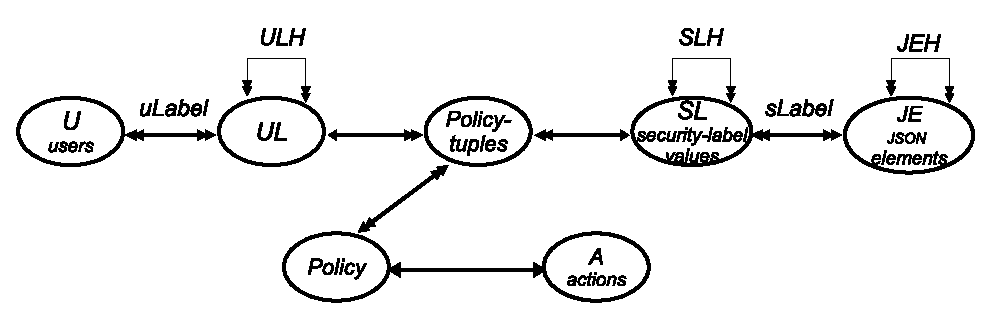
\includegraphics[width=.9\textwidth]{NSS16/operational-model}
 		\caption{ The Attribute-based Operational Model (\atom{})}
 		\label{fig:operational-model}
 	\end{figure}
 


\label{sec:operational-model}


This section presents the Attribute-based Operational Model (\atom{}) for protection of JSON documents. \atom{} adapts enumerated authorization policies from  \cite{labac,eap-abac}.


\begin{table}[t]
	\centering
	\caption{ Definition of \atom{}} %\vspace*{3pt}
	\label{tab:operational-model}			
	\begin{tabular}{|l|}

		\hline					
				\begin{tabular}{l}
							\multicolumn{1}{c}{\underline{\textit{I. Sets and relations }}}\\			
							- \textit{U, JE} and $A$  (set of users, JSON elements and actions respectively)  \\
							- \textit{JEH} (hierarchy of JSON elements, represented by $\JEH$) \\
							- \textit{UL} and \textit{ULH} (finite set of uLabel values and their partial order denoted as $\udominate$ respectively) \\
							- \textit{SL} and  \textit{SLH} (finite set of security-label values and their partial order denoted as $\odominate$ respectively) \\
							- $\uLabel$ and $sLabel$ (attribute functions on users and JSON objects respectively) \\
							 \hfil Formally, $\uLabel: U \to 2^{UL}$; $\oLabel: JO \to 2^{SL}$ \\														

							 \multicolumn{1}{c}{\underline{\textit{II. Policy components}}} \\	
							 - $\policyTuples{} = UL \times SL$\\			
							- $Policy_a \subseteq \policyTuples{}$ for $a \in A$ \\
							-  $Policy = \{Policy_a | a \in A\}$ \\
							\multicolumn{1}{c}{\underline{\textit{III. Authorization function}}} \\						
							%- $\request(u:U, a:A, je_i:JE)$ =	($\forall je_j \preceq je_i$ ($\exists ul_i \in \uLabel(u), \exists sl_m \in \oLabel(je_j),$ \\ \hfill$\exists (ul_j, sl_n) \in Policy_a $) ) $[ul_i \udominate ul_j \land sl_m \odominate sl_n]$ 
							- $\canAccess (u:U, a:A, o:JE) =  (\exists (ul,sl) \in Policy_a) [ul \in \uLabel(u) \land sl \in \oLabel(o)]$\\
							- $\request(u:U, a:A, je_i: JE) \equiv \exists je_j [(\canAccess(u,a,je_j)) \land je_i \odominate je_j]$ \\
							
				\end{tabular}
					
			
 \\ \hline	
	\end{tabular}
	
\end{table}



  	\begin{figure} [t]
 		\centering
 		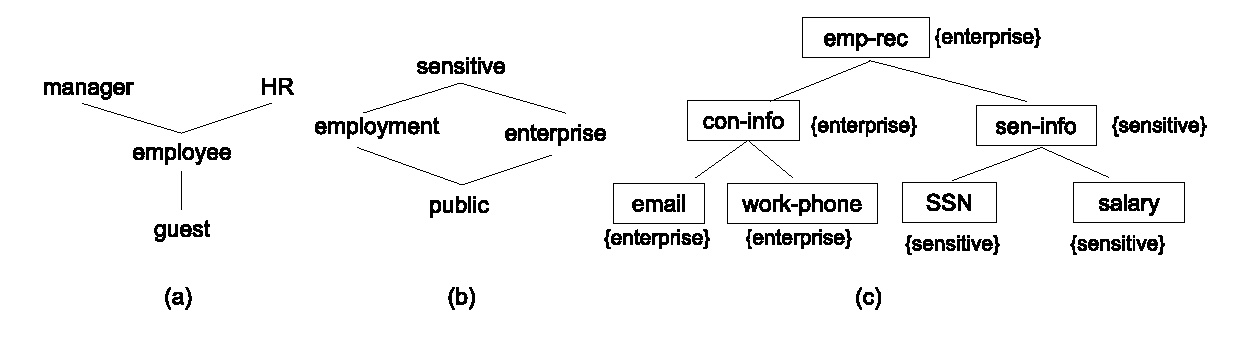
\includegraphics[width=1\textwidth]{NSS16/operational-explanation}
 		\caption{(a) User-label values, (b) Security-label values and (c)  Annotated JSON tree}
 		\label{fig:operational-explanation}
 	\end{figure}
 
\begin{table}[t]
\centering
\caption{Example of an authorization policy and authorization requests}
\label{tab:example-auth-policy}
\begin{tabular}{|l|}
	\hline
%\textit{}                      \\ \hline
\multicolumn{1}{|c|}{\textit{\underline{I. Enumerated authorization policies}}} \\   
$Policy_{read} \equiv$ \{ \textit{(manager,sensitive), (HR,employment)}, \\ \hfill \textit{(employee, enterprise), (guest, public)}\}\\ \hline

\multicolumn{1}{|c|}{\textit{\underline{II. Authorization requests}}} \\   
$\request(Alice,read, \textit{emp-rec}) = true$, assuming $\uLabel(Alice)=\{manager\}$\\
$\request(Bob,read, \textit{emp-rec}) = false$, assuming $\uLabel(Bob)=\{employee\}$\\
$\request(Bob,read, \textit{con-info}) = true$, assuming $\uLabel(Bob)=\{employee\}$\\
$\request(Charlie,read, \textit{sen-info}) = false$, assuming $\uLabel(Charlie)=\{HR\}$\\
\hline
\end{tabular}
\end{table}


%$ Policy_{read} \equiv \{(Visitors, public\_data), (HR, persona\_data),(HR, employment\_data),$  \\\hfil $(employee, protected\_data),(manager,sensitive\_data)\}$         \\ \hline
%$Policy_{write} \equiv \{(HR, personal\_data),(HR, employment\_data),$ \\ \hfil $(director, sensitive\_data)\}$ \\ \hline

Figure \ref{fig:operational-model} presents components of \atom{}. In the figure, the set of users is represented by $U$. Each user is assigned to one or more values of an attribute named \textit{user-label} or \textit{uLabel} in short. These values are selected from the set of all possible user-label values $UL$ which are partially ordered. The partial order is represented by $ULH$. An example showing user-label values and  hierarchy is presented in Figure \ref{fig:operational-explanation}(a). On the other hand, the set of JSON elements are specified as \textit{JE}. JSON elements may subsume other JSON elements, and form a tree structured hierarchy. The hierarchy is represented by \textit{JEH}. Each JSON element is assigned values of an attribute named \textit{security-label} or \textit{sLabel} in short. These values are selected from the set of security-label values $SL$ which are also partially ordered. The partial order is represented by \textit{SLH}. An example showing security-label values and  hierarchy is presented in Figure \ref{fig:operational-explanation}(b). A JSON tree annotated with security-label values is given in Figure \ref{fig:operational-explanation}(c). These components and relationship among them are formally specified in Segment I of Table  \ref{tab:operational-model}.

% The many-to-many relation between JSON elements and security-label values are specified by the attribute function \textit{sLabel}In an organization, it is possible to have an existing classification system that categorizes all objects or resources in the organization. Such a classification system can be used to derive security-label values and its hierarchy. 

In Figure \ref{fig:operational-model}, the set of authorization policies is represented by \textit{Policy}. There exists one authorization policy per action which is shown by the one-to-one relation between  \textit{Policy} and the action \textit{A}. In Table \ref{tab:operational-model}, $Policy_{read}$ presents the authorization policy for  action read. An authorization policy may contain one or more micro-policies, and one micro-policy can be associated with more than one authorization policy. This is represented by the many-to-many relation between \textit{Policy} and \textit{Policy-tuples}. $Policy_{read}$, as mentioned above, contains four policy-tuples including \textit{(manager, sensitive)}. The tuple \textit{(manager, sensitive)} in policy $Policy_{read}$ specifies that users who are manager can read objects that have been assigned values sensitive. Formally, we represent a policy-tuple as a pair of atomic values $(ul, sl)$ where $ul \in UL$ and $sl \in SL$. The formal definition of policies and policy-tuples is given in Segment II of Table \ref{tab:operational-model}. We use the terms policy-tuples and micro-policies equivalently to represent sub-policies.

%The formal definition of \atom{} is given in Table \ref{tab:operational-model}. In Section I of the table, we formally specify the sets and relations used in the model as described above. Section II formally specifies the relationship among policies, actions and policy-tuples. 

The authorization function $\request{}()$ is specified in Section III of Table \ref{tab:operational-model}. We define the helper function $\canAccess{}(u,a,o)$ which specifies that the user $u$ can access the object $o$ for action $a$ if there exists a policy-tuple in $Policy_{a}$ that allows it. A user is authorized to perform an action on the requested JSON element  if he can access the requested element and all its sub-elements. For example, let us assume, Alice as a manager wants to read \textit{emp-rec} which has been assigned value \textit{enterprise} as shown in Figure \ref{fig:operational-explanation}(c). The tuple \textit{(manager, sensitive)} in $Policy_{read}$ specifies that Alice can read object labeled with sensitive or junior values. Thus, the request $\request$\textit{(Alice, read, emp\_rec)} is evaluated as true. On the other hand, assuming Bob as an employee, the request \textit{\request(Bob, read, emp-rec)} is evaluated as false as an employee cannot read \textit{sen-info} which is sub-element of \textit{emp-rec}. Additional examples of authorization request are given in Segment II of Table  \ref{tab:example-auth-policy}.


